% Copyright 2020 by Junwei Wang <i.junwei.wang@gmail.com>
%
% This file may be distributed and/or modified under the
% conditions of the LaTeX Project Public License, either version 1.3c
% of this license or (at your option) any later version.
% The latest version of this license is in
%   http://www.latex-project.org/lppl.txt

%\newcommand{\ar}{43}
\newcommand{\ar}{1610}
\documentclass[compress,aspectratio=\ar]{beamer}
%\documentclass[handout,compress,aspectratio=\ar]{beamer} % disable \pause temporarily

\usepackage[english]{babel}
\usepackage{csquotes}
%\usepackage[dvipsnames]{xcolor}
\usepackage{metalogo}
\usepackage{fontspec}
\usepackage{hyperref}
 
\usepackage{listings}
\usepackage{algorithm}
\usepackage{algpseudocode}

\usepackage{booktabs}
\usepackage{wasysym}

\usepackage{graphicx}
\usepackage{subcaption}
\usepackage{xfp}

\usepackage{fontawesome5} %for icons 

\usepackage{multirow}

\usepackage{tikz}
\usepackage{tikzpeople} 
\usepackage{pgfplots} \pgfplotsset{compat=1.18}
\usepackage{tikz}
\usetikzlibrary{positioning}
\usetikzlibrary{arrows}
\usetikzlibrary{calc} %%
%https://tex.stackexchange.com/questions/23536/how-can-you-position-a-node-relatively-to-another-in-tikz
\usetikzlibrary {shapes.multipart}
\usetikzlibrary {shapes.geometric}
\usetikzlibrary{patterns}
\usetikzlibrary{decorations.markings}
\usetikzlibrary{decorations.pathreplacing}
\usetikzlibrary{calligraphy}
\usetikzlibrary{overlay-beamer-styles}
\usetikzlibrary{fadings}
\usepackage{circuitikz}

%\tikzstyle{window} = [rectangle, rounded corners, text centered, draw=black, fill=white, minimum width = 10cm, minimum height = 8cm, anchor=south west]

%\tikzstyle{other} = [rectangle, rounded corners, text centered, draw=black, fill=white, anchor=south west, minimum width=#1 cm, minimum height=#2 cm]

% Scaling factor
%\newcommand\scalingFactorTikz{0.45}

% To resize TikZ picture with resizebox
\newcommand\resizeTB[2]{\scalebox{#1\linewidth}{!}{#2}}
\newcommand\resizeTikz[1]{\resizebox{0.45\linewidth}{!}{#1}}

% Create the window
\newcommand\drawWindow{
    %\draw[draw=white, fill=black!10] (0,9) [sharp corners] -- (0,10) [rounded corners] -- (14,10) [rounded corners] -- (14,9) [sharp corners];
    \node[window] at (0,0) {};
    \node[entry={10cm}{0.6cm}] at (0.25,9.5) {};
    \draw (0,9) -- (14,9);
}

% For TikZ styles
\tikzset{
% for every node
every text node part/.style={align=center},
every node/.style={outer sep=0pt}, % avoid anchor being a bit shifted
% text-only node
text_only/.style={anchor=west},
% rounded block node
r_block/.style 2 args={rectangle, rounded corners, text centered, draw=black, fill=white, minimum width = #1, minimum height = #2, anchor=west},
% sharp block node
s_block/.style 2 args={rectangle, text centered, draw=black, fill=white, minimum width = #1, minimum height = #2, anchor=west},
memory/.style={rectangle split, rectangle split parts=4, rectangle split part align=center, draw=black, thin, text width=2.5cm, text centered, execute at begin node=\strut, outer sep=2pt}
}

\tikzset{
    make origin horizontal center of bounding box/.style={%
        execute at end picture={%
            \path
                let 
                    \p1=(current bounding box.west),
                    \p2=(current bounding box.east)
                    in ({-max(-1*\x1,\x2)},\y1) ({max(-1*\x1,\x2)},\y1);
        }
    }
}

\newcommand{\scopedrawsequence}[9][]{
    \begin{scope}
        \foreach \idx/\val [count=\yi from 0]
            in {0/#2, 1/#3, 2/#4, 3/#5, 4/#6, 5/#7, 6/#8, 7/#9}
        {
            \node (\idx) at (#1,-\yi) {\val};
        }
        \draw[->]
            (0) edge (1)
            (1) edge (2)
            (2) edge (3)
            (3) edge (4)
            (4) edge (5)
            (5) edge (6)
            (6) edge (7);
    \end{scope}
}


\usepackage{relsize} % for \mathlarger
\usetikzlibrary{overlay-beamer-styles, shapes.geometric, positioning, calc, patterns, patterns.meta, backgrounds, fit, decorations.pathreplacing}

\definecolor{background}{HTML}{ffffff}
\definecolor{lightorange}{HTML}{FFE5CC}
\definecolor{highlight}{HTML}{ed7014} % #ed7014
\colorlet{unhighlight}{background!40!gray}
\colorlet{unHighlight}{background!40!gray}
% \definecolor{unHighlight}{gray}{0.60}
\colorlet{color1}{blue}
\colorlet{color2}{red}
\colorlet{color3}{green}
\definecolor{rainbow1}{HTML}{1E6F91} % #1E6F91
\definecolor{rainbow2}{HTML}{3AA9B3} % #3AA9B3
\definecolor{rainbow3}{HTML}{56C2AE} % #56C2AE 
\definecolor{rainbow4}{HTML}{B5E48C} % #B5E48C 
\definecolor{rainbow5}{HTML}{FFD166} % #FFD166 
\definecolor{rainbow6}{HTML}{FF9F68} % #FF9F68 
\definecolor{rainbow7}{HTML}{FFB6C1} % #FFB6C1 



\setbeamertemplate{enumerate item}{%
  \tikz[baseline=(b.base)]
    \node[eq, fill=white] (b) {\footnotesize\insertenumlabel};%
}

\newcommand{\x}{7mm}
\newcommand{\yy}{5mm}

\newlength{\y}
\newcommand{\width}{9mm}
\newcommand{\height}{5.4mm}

\newcommand{\vgap}{
    \addtolength{\y}{-\height}
    \addtolength{\y}{-1mm}
}
\newcommand{\vGap}{
    \addtolength{\y}{-\height}
    \addtolength{\y}{-3mm}
}


\newcommand{\size}{\normalsize}
\newcommand{\subsize}{\tiny}

% Handle text and math mode consistent notation
\newcommand{\inmath}[1]{\relax\ifmmode \text{\size $#1$} \else {\size $#1$} \fi}
\renewcommand{\index}[1]{\relax\ifmmode {\mathrm{\text{\subsize #1}}} \else {\text{\subsize #1}} \fi}
% \renewcommand{\index}[1]{ %
%   \ifdim \y > 2mm
%     \mathrm{\text{\normalsize #1}}%
%   \else
%     \mathrm{\text{\tiny #1}}%
%   \fi
% }

\newcommand{\sk}[1]{\inmath{k_\index{#1}}}
% \newcommand{\PK}[1]{\inmath{K_\index{#1}}}
\newcommand{\N}[1]{\inmath{N_\index{#1}}}
\renewcommand{\S}[2]{\inmath{S_\index{#1#2}}}

% Generators
\newcommand{\G}[1]{\inmath{G_\index{#1}}}
\newcommand{\s}[1]{\relax\ifmmode s_{\raisebox{-0.1mm}{\subsize #1}} \else $s_{\raisebox{-0.1mm}{\hspace{0.1mm}\subsize #1}}$ \fi}
\newcommand{\sG}[2] {\relax
    \ifmmode \s{#1}\G{#2} 
    \else $\s{#1}\textcolor{unHighlight}{\G{#2}}$ 
\fi}
\newcommand{\sGcolored}[4]{\inmath{{\color{#3}s_\index{#1}}{\color{#4}G_\index{#2}}}}

% Alpha, Beta, Gamma, Delta
\newcommand{\A}[1]{\relax\ifmmode \alpha_{\raisebox{-0.4mm}{\subsize #1}} \else $\alpha_{\raisebox{-0.4mm}{\subsize #1}}$ \fi}
% \newcommand{\B}[2]{\inmath{\beta_\index{#1#2}}}
% \newcommand{\Bprime}[2]{\inmath{\beta^\prime_\index{#1#2}}}
% \newcommand{\BB}[2]{\relax
%     \ifmmode \mathlarger{\beta^\prime_\index{#1#2}} 
%     \else $\mathlarger{\beta^\prime_\index{#1\textcolor{unHighlight}{#2}}}$ 
% \fi}
\newcommand{\B}[2]{\relax
    \ifmmode \mathlarger{\beta_\index{#1#2}} 
    \else $\mathlarger{\beta_\index{#1\textcolor{unHighlight}{#2}}}$ 
\fi}
\newcommand{\BB}[2]{\relax
    \ifmmode \mathlarger{\beta^\prime_\index{#1#2}} 
    \else $\mathlarger{\beta^\prime_\index{#1\textcolor{unHighlight}{#2}}}$ 
\fi}
\newcommand{\C}[1]{\relax\ifmmode \gamma_{\raisebox{-0.7mm}{\subsize #1}} \else $\gamma_{\raisebox{-0.7mm}{\subsize #1}}$ \fi}
\newcommand{\D}{\inmath{\mathrm{\Delta}}}

% Hashes and Mappings
\newcommand{\hash}[1]{\inmath{\mathnormal{h}(#1)}}
\newcommand{\sHashed}[1]{\inmath{\sigma_\index{#1}}}
\newcommand{\hashIt}[2]{\inmath{\mathsf{h}^{(#2)}(#1)}}
\newcommand{\Map}[1]{\inmath{\mathsf{Map}(#1)}}
\newcommand{\InverseMap}[1]{\inmath{\mathsf{Map}^{-1}(#1)}}


\newcommand{\at}[3]{\node at ($(#1.west) + ({#2*\x}, {-#3*\yy})$)}
\newcommand{\highlightEnter}[1]{
    \only<\thebeamerpauses>{{\color{highlight}#1}}
    \only<\thebeamerpausesplusONE->{{\color{black}#1}}
}
\newcommand{\highlightExit}[1]{
    \only<\thebeamerpauses>{{\color{highlight}#1}}
}

\newcounter{beamerpausesplusONE}\setcounter{beamerpausesplusONE}{1}
\newcounter{beamerpausesplusTWO}\setcounter{beamerpausesplusTWO}{2}
\newcounter{beamerpausesplusTHREE}\setcounter{beamerpausesplusTHREE}{3}
\newcommand{\updatebeamerpauses}[1]{
    \setcounter{beamerpauses}{#1}
    \setcounter{beamerpausesplusONE}{\value{beamerpauses}+1}
    \setcounter{beamerpausesplusTWO}{\value{beamerpauses}+2}
    \setcounter{beamerpausesplusTHREE}{\value{beamerpauses}+3}
}
\newcommand{\incrementAnimation}{
    \stepcounter{beamerpauses}
    \setcounter{beamerpausesplusONE}{\value{beamerpauses}+1}
    \setcounter{beamerpausesplusTWO}{\value{beamerpauses}+2}
    \setcounter{beamerpausesplusTHREE}{\value{beamerpauses}+3}
}
\newcommand{\slide}[2]{%
  \only<\thebeamerpauses-
  \ifcase#1 \thebeamerpauses
  \or \thebeamerpausesplusONE % case 1
  \or \thebeamerpausesplusTWO % case 2
  \or \thebeamerpausesplusTHREE % case 3
  \else\PackageError{slide}{Invalid argument #2}{Use 0--3 only}
  \fi
  >{{#2}}
}

\newcommand{\patternA}[3]{ 
    \node at ($(#1.west) + ({#2*\x - \x}, 0)$) [p1=#3] {};
    \node at ($(#1.west) + ({#2*\x - \x}, 0)$) [c1=#3] {};
}\newcommand{\patternB}[3]{ 
    \node at ($(#1.west) + ({#2*\x - \x}, 0)$) [p2=#3] {};
    \node at ($(#1.west) + ({#2*\x - \x}, 0)$) [c2=#3] {};
}\newcommand{\patternC}[3]{ 
    \node at ($(#1.west) + ({#2*\x - \x}, 0)$) [p3=#3] {};
    \node at ($(#1.west) + ({#2*\x - \x}, 0)$) [c3=#3] {};
}\renewcommand{\patterns}[7]{ 
    \patternA{#1}{#2}{#3}
    \patternB{#1}{#4}{#5}
    \patternC{#1}{#6}{#7}
}


\tikzset{    
    % shape
    block/.style={minimum width = #1*\x, minimum height = 0.85*\yy, inner sep = 0mm, anchor=west},%
    inblock/.style={minimum width = #1*\x - 0.16mm, minimum height = 0.85*\yy - 0.35mm, xshift=0.08mm, inner sep = 0mm, anchor=west},
    zero_pad/.style={block = #1, fill = unhighlight, fill opacity=0.3, font=\size},%
    HMAC/.style={draw, ellipse, fill = background, minimum width = \x, minimum height = \y, inner sep = 0mm, anchor = center},%
    eq/.style={draw, circle, inner sep=0.35mm, fill=lightorange}, %font=\bfseries\large
    arrow/.style={->, shorten <= 0.35mm, shorten >= 0.7mm, -{Classical TikZ Rightarrow[length=0.7mm]}},%%   -{Stealth[length=4pt]} 
    line/.style={shorten <= 0.35mm, shorten >= 0.35mm},
    between/.style args={#1 and #2}{at = ($(#1)!0.5!(#2)$)},
    % Pattern
    pattern1/.style={pattern = {Lines[angle=45, distance=6pt, line width=2pt, xshift= 0pt]}, pattern color = color1, opacity = 0.4},
    pattern2/.style={pattern = {Lines[angle=45, distance=6pt, line width=2pt, xshift= 3pt]}, pattern color = color2, opacity = 0.4},
    pattern3/.style={pattern = {Lines[angle=45, distance=6pt, line width=2pt, xshift= 6pt]}, pattern color = color3, opacity = 0.4},
    fill1/.style={fill = color1,        opacity = 0.2},
    fill2/.style={fill = color2,        opacity = 0.2},
    fill3/.style={fill = color3,        opacity = 0.2},
    % Color
    p1/.style={inblock = #1, pattern = {Lines[angle=45, distance=3pt, line width=1pt, xshift=  0mm]}, pattern color = color1, opacity = 0.4},
    p2/.style={inblock = #1, pattern = {Lines[angle=45, distance=3pt, line width=1pt, xshift=1.5pt]}, pattern color = color2, opacity = 0.4},
    p3/.style={inblock = #1, pattern = {Lines[angle=45, distance=3pt, line width=1pt, xshift=  3pt]}, pattern color = color3, opacity = 0.4},
    p0/.style={},
    c1/.style={inblock = #1,                                      fill = color1,        opacity = 0.2},
    c2/.style={inblock = #1,                                      fill = color2,        opacity = 0.2},
    c3/.style={inblock = #1,                                      fill = color3,        opacity = 0.2},
    c0/.style={inblock = #1,                                      fill = unhighlight,   opacity = 0.2},
    unused/.style={inblock = #1, fill=unhighlight!30},
}

\newcommand\Warning{%
  \makebox[2em][c]{%
    \makebox[0mm][c]{\raisebox{.25em}{\bfseries\Large!}}%
    \makebox[0mm][c]{\color{red}\scalebox{3}{$\bigtriangleup$}}}}




\tikzset{
  on/.style={
    alt=<#1>{highlight!60, very thick}{}
  },
  hightOn/.style={
    alt=<#1>{fill=highlight!35}{}
  },
  mHightOn/.style={
    alt=<#1->{highlight}{},
    alt=<#1>{fill=highlight!35}{},
  }
}
\usetikzlibrary{arrows.meta, positioning, backgrounds, shapes.arrows}
\usetikzlibrary{decorations.pathreplacing,calc} % TODO ?
\usetikzlibrary{fit}
%\usetheme{Nord}
\usetheme[style=light]{Nord}
 
\setmainfont{Yanone Kaffeesatz}
\setsansfont{Andika New Basic}
\setmonofont{DejaVu Sans Mono}

\newcommand{\server}[1]{
  \begin{tikzpicture}[scale=0.7]
    \foreach \y in {0, -0.6, -1.2} {
        \draw[fill=#1!20] (0,\y) rectangle (2,\y-0.5); % rectangle
        \draw (0.2,\y-0.25) circle (0.05); % power/status LED
    }
  \end{tikzpicture}
}
\newcommand{\client}[1]{
  \begin{tikzpicture}[scale=0.4]
    % Monitor screen
    \draw[fill=#1!20, draw=black, rounded corners=4pt] (0,0) rectangle (4,2.5);
    % Inner bezel
    \draw[fill=white, draw=none, rounded corners=3pt] (0.2,0.2) rectangle (3.8,2.3);
    % Stand
    \draw[fill=#1!40, draw=black] (1.75,-0.7) rectangle (2.25,0);
    % Base
    \draw[fill=#1!40, draw=black, rounded corners=2pt] (0.8,-1) rectangle (3.2,-0.7);
  \end{tikzpicture}
}
\tikzset{  
    innerLink/.style={-, densely dotted, shorten <= 1pt, shorten >= 2pt},  
    outerLink/.style={->, shorten <= 10pt, shorten >= 10pt, >=Latex},
    packet/.style={circle, minimum size=3mm, inner sep=0.2pt, fill=#1!35},
    mixnode/.style={draw, thick, circle, minimum size=1.6cm},
}



\definecolor{LightHighlight}{HTML}{AEC0D5} 
\definecolor{MidHighlight}{HTML}{5E81AC}
\definecolor{Highlight}{HTML}{204B82}
\setbeamercolor{block title}{
    fg=Highlight,
    bg=MidHighlight!50
}

\setbeamercolor{block body}{
    fg=black,
    bg=LightHighlight!50
}


% \AtBeginSection[]
% {
%   \begin{frame}[c,noframenumbering,plain,sectionbackground]
%     \tableofcontents[sectionstyle=show/shaded,subsectionstyle=hide]
%   \end{frame}
% }

\AtBeginSection[]{
  \nordnavoff
  \begin{frame}[c,noframenumbering,plain,sectionbackground]
    \tableofcontents[
      sectionstyle=show/shaded,
      subsectionstyle=hide
    ]
  \end{frame}
  \nordnavon
}

\AtBeginSubsection[]
{
  \begin{frame}[c,noframenumbering,plain,sectionbackground]
    \tableofcontents[sectionstyle=show/hide,subsectionstyle=show/shaded/hide]
  \end{frame}
}


\makeatletter
%% reset ToC
\@addtoreset{section}{part}

%% reset frame number
% source: https://tex.stackexchange.com/questions/278873/how-to-reset-frame-number-in-beamer-correctly-when-using-parts
\newcount\beamer@partstartframe
\beamer@partstartframe=1
\apptocmd{\beamer@part}{\addtocontents{nav}{\protect\headcommand{%
    \protect\beamer@partframes{\the\beamer@partstartframe}{\the\c@framenumber}}}}{}{}
\apptocmd{\beamer@part}{\beamer@partstartframe=\c@framenumber\advance\beamer@partstartframe by1\relax}{}{}
\AtEndDocument{\immediate\write\@auxout{\string\@writefile{nav}%
    {\noexpand\headcommand{\noexpand\beamer@partframes{\the\beamer@partstartframe}{\the\c@framenumber}}}}}{}{}
\def\beamer@startframeofpart{1}
\def\beamer@endframeofpart{1}
\def\beamer@partframes#1#2{%
    \ifnum\c@framenumber<#1%
    \else%
    \ifnum\c@framenumber>#2%
    \else%
    \gdef\beamer@startframeofpart{#1}%
    \gdef\beamer@endframeofpart{#2}%
    \fi%
    \fi%
}
\newcommand\insertpartstartframe{\beamer@startframeofpart}
\newcommand\insertpartendframe{\beamer@endframeofpart}


%% Do not add section-TOC frames to the Nord navigation/smoothbar
\let\beamer@writeslidentry@normal=\beamer@writeslidentry

\def\beamer@writeslidentry@nonav{%
    \expandafter\beamer@ifempty\expandafter{\beamer@framestartpage}{}%
    {%
        \clearpage
        \beamer@notesactions
    }%
}

\newcommand{\nordnavoff}{%
    \let\beamer@writeslidentry=\beamer@writeslidentry@nonav
}

\newcommand{\nordnavon}{%
    \let\beamer@writeslidentry=\beamer@writeslidentry@normal
}

\tikzset{
  appears/.style args={#1}{
    color/.expanded={
      \ifnum\beamer@slideinframe<#1
        white%
      \else\ifnum\beamer@slideinframe=#1
        alerted text.fg%
      \else
        LightHighlight%
      \fi\fi
    },
    opacity/.expanded={
      \ifnum\beamer@slideinframe<#1
        0%
      \else\ifnum\beamer@slideinframe=#1
        1%
      \else
        1%
      \fi\fi
    }
  },
  highlight/.style args={#1}{
    color/.expanded={
      \ifnum\beamer@slideinframe<#1
        black%
      \else\ifnum\beamer@slideinframe=#1
        alerted text.fg%
      \else
        LightHighlight%
      \fi\fi
    }
  },
  visible/.style args={#1}{
    opacity/.expanded={
      \ifnum\beamer@slideinframe<#1
        0%
      \else\ifnum\beamer@slideinframe=#1
        1%
      \else
        0%
      \fi\fi
    }
  },
  on/.style args={#1}{
    color/.expanded={
      \ifnum\beamer@slideinframe<#1
        white%
      \else\ifnum\beamer@slideinframe=#1
        alerted text.fg%
      \else
        black%
      \fi\fi
    }
  },
  on_MidHighlight/.style args={#1}{
    color/.expanded={
      \ifnum\beamer@slideinframe<#1
        white%
      \else\ifnum\beamer@slideinframe=#1
        alerted text.fg%
      \else
        MidHighlight%
      \fi\fi
    }
  },
}
\makeatother
\def\inserttotalpartframenumber{%
    %\pgfmathparse{(\insertpartendframe-\insertpartstartframe+1)}%
    %\pgfmathprintnumber[fixed,precision=2]{\pgfmathresult}%
    \fpeval{\insertpartendframe-\insertpartstartframe+1}%
}

\def\insertpartframenumber{%
    %\pgfmathparse{(\insertframenumber-\insertpartstartframe+1)}%
    %\pgfmathprintnumber[fixed,precision=2]{\pgfmathresult}%
    \fpeval{\insertframenumber-\insertpartstartframe+1}%
}



\title{DSphinx: A Decentralized Path Selection \newline for Decentralized Networks} 
% \subtitle{Subtitle}
\author{Aurélien Chassagne}
\date{\today}
  

%\newcommand\highlight[1]{\textbf{\textcolor{ColorStructure}{#1}}}
\newcommand\highlight[1]{\textcolor{ColorStructure}{#1}}

\lstset{
frame               = single,
%framexleftmargin    = 15pt,
%tabsize             = 4,
breaklines          = true,
%breakatwhitespace   = true,
%numbers             = left,
%    numberstyle     = \tiny,
basicstyle          = \ttfamily\tiny,
%keywordstyle        = \lst@ifdisplaystyle\bfseries\fi\color{blue!70},
%commentstyle        = \color{comment-green}\upshape,
%stringstyle         = \color{red},
%identifierstyle     = \color[rgb]{0.1,0.1,0.1},
%rulecolor           = \color{black}
}


\newcommand\arrowitem{\smallskip\item[$\rightarrow$]}
\newcommand\triangleitem{\smallskip\item[$\blacktriangleright$]}
%different skips: \smallskip, \medskip, \bigskip

\newcommand{\mycomment}[1]{}
\newcommand\mathacro[1]{\mathrm{\mathit{#1}}}

\newcommand\cred[1]{\textcolor{red}{#1}}
\newcommand\cgreen[1]{\textcolor{green}{#1}}
\newcommand\OK{\cgreen{\faIcon{check}}}
\newcommand\notOK{\cred{\faIcon{times}}}

\newcommand\hlg[1]{\colorbox{gray!25}{#1}}
\newcommand\hlgl[1]{\colorbox{gray!15}{#1}}

\begin{document}

%%% part 1
\part{} % used to clean ToC later
\def\slidepart{0}
\begin{frame}[plain,noframenumbering,titlebackground]
    \maketitle
\end{frame}

\begin{frame}[plain,noframenumbering,sectionbackground]%{Table of Contents}
    \tableofcontents[subsectionstyle=hide]
\end{frame}

\section{Problem Statement} 
\begin{frame}{Introduction}

\vspace{8mm}

\resizebox{\linewidth}{!}{
  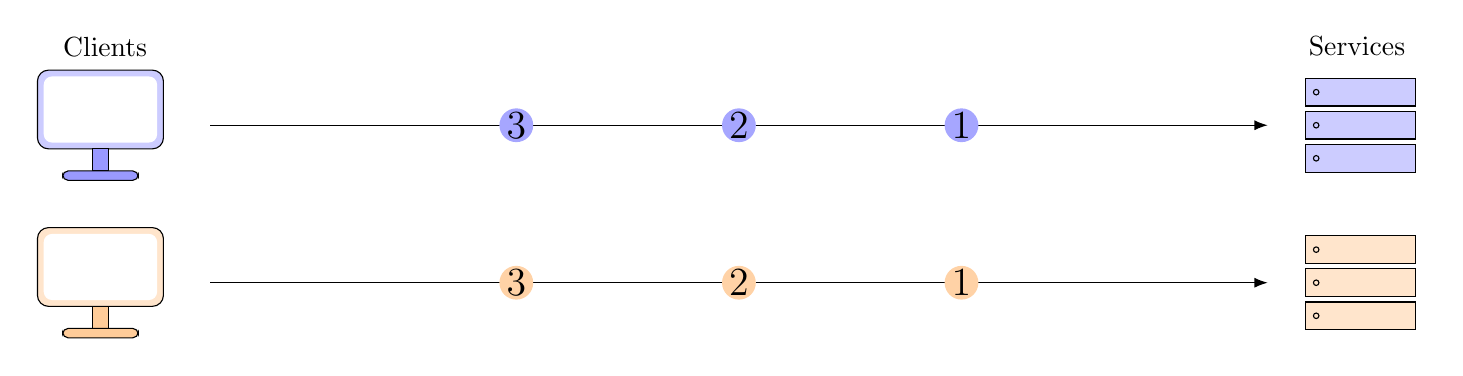
\begin{tikzpicture}
      \def\dx{4}
      \def\high{-1}
      \def\low{-3}

  %------------------------------------------------
  % LEFT COLUMN — CLIENTS
  %------------------------------------------------
  \node (C1) at (0,\high) {\client{blue}};
  \node (C2) at (0,\low) {\client{orange}};

  \node at (0,0) {Clients};

  %------------------------------------------------
  % RIGHT COLUMN — SERVICES
  %------------------------------------------------
  \node (S1) at (4*\dx,\high) {\server{blue}};
  \node (S2) at (4*\dx,\low) {\server{orange}};

  \node[xshift=-1mm] at (4*\dx,0) {Services};


  %------------------------------------------------
  % Packets
  %------------------------------------------------
  \draw[outerLink] (C1.east) -- 
    node[pos=0.3,packet=blue]{\Large 3}  
    node[pos=0.5,packet=blue]{\Large 2}  
    node[pos=0.7,packet=blue]{\Large 1}  
    (S1.west); 

  \draw[outerLink] (C2.east) -- 
    node[pos=0.3,packet=orange]{\Large 3}  
    node[pos=0.5,packet=orange]{\Large 2}  
    node[pos=0.7,packet=orange]{\Large 1}  
    (S2.west); 

  \end{tikzpicture}
}

\vspace{10mm}

\begin{center}
  \textbf{Despite encryption, metadata reveals who is communicating to whom}
\end{center}



\end{frame}
\begin{frame}{Mixnet: A Privacy-Preserving Network}

% \begin{center}
%   Mixnet packets are routed through intermediate nodes hiding the sender-recipient relationship
% \end{center}

\vspace{10mm}

\resizebox{\linewidth}{!}{
  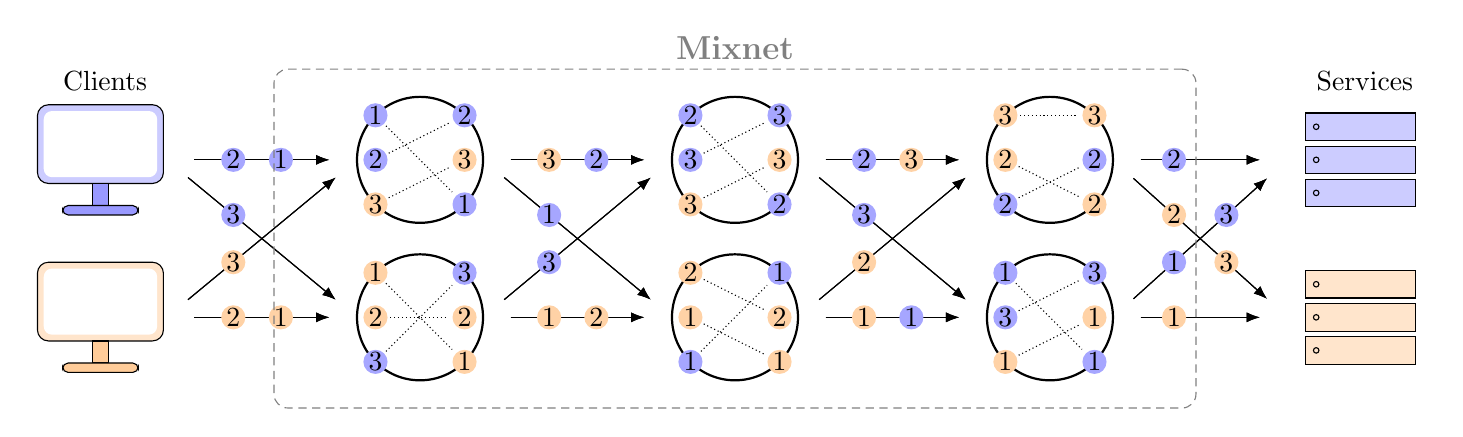
\begin{tikzpicture}
      \def\dx{4}
      \def\high{-1}
      \def\low{-3}

  %------------------------------------------------
  % LEFT COLUMN — CLIENTS
  %------------------------------------------------
  \node (C1) at (0,\high) {\client{blue}};
  \node (C2) at (0,\low) {\client{orange}};

  \node at (0,0) {Clients};

  %------------------------------------------------
  % RIGHT COLUMN — SERVICES
  %------------------------------------------------
  \node (S1) at (4*\dx,\high) {\server{blue}};
  \node (S2) at (4*\dx,\low) {\server{orange}};

  \node at (4*\dx,0) {Services};

  %------------------------------------------------
  % mix1
  %------------------------------------------------
  \node[mixnode] (mix11) at (1*\dx,\high) {};
  \node[mixnode] (mix12) at (1*\dx,\low) {};

  \onslide<3->{
  \begin{scope}[alt=<4->{opacity=0.3}{opacity=1}]
  \node[packet=blue] (l1) at (mix11.135) {1};
  \node[packet=blue] (l2) at (l1 |- mix11) {2};
  \node[packet=orange] (l3) at (mix11.225) {3};

  \node[packet=blue] (r2) at (mix11.45) {2};
  \node[packet=orange] (r3) at (r2 |- mix11) {3};
  \node[packet=blue] (r1) at (mix11.-45) {1};

  \draw[innerLink] (l1) -- (r1);
  \draw[innerLink] (l2) -- (r2);
  \draw[innerLink] (l3) -- (r3);


  \node[packet=orange] (l1) at (mix12.135) {1};
  \node[packet=orange] (l2) at (l1 |- mix12) {2};
  \node[packet=blue] (l3) at (mix12.225) {3};

  \node[packet=blue] (r3) at (mix12.45) {3};
  \node[packet=orange] (r2) at (r3 |- mix12) {2};
  \node[packet=orange] (r1) at (mix12.-45) {1};

  \draw[innerLink] (l1) -- (r1);
  \draw[innerLink] (l2) -- (r2);
  \draw[innerLink] (l3) -- (r3);
  \end{scope}
  }

  %------------------------------------------------
  % mix2
  %------------------------------------------------
  \node[mixnode] (mix21) at (2*\dx,\high) {};
  \node[mixnode] (mix22) at (2*\dx,\low) {};

  \onslide<5->{
  \begin{scope}[alt=<6->{opacity=0.3}{opacity=1}]
  \node[packet=blue] (l1) at (mix21.135) {2};
  \node[packet=blue] (l2) at (l1 |- mix21) {3};
  \node[packet=orange] (l3) at (mix21.225) {3};
  
  \node[packet=blue] (r2) at (mix21.45) {3};
  \node[packet=orange] (r3) at (r2 |- mix21) {3};
  \node[packet=blue] (r1) at (mix21.-45) {2};

  \draw[innerLink] (l1) -- (r1);
  \draw[innerLink] (l2) -- (r2);
  \draw[innerLink] (l3) -- (r3);


  \node[packet=orange] (l1) at (mix22.135) {2};
  \node[packet=orange] (l2) at (l1 |- mix22) {1};
  \node[packet=blue] (l3) at (mix22.225) {1};

  \node[packet=blue] (r3) at (mix22.45) {1};
  \node[packet=orange] (r1) at (r3 |- mix22) {2};
  \node[packet=orange] (r2) at (mix22.-45) {1};

  \draw[innerLink] (l1) -- (r1);
  \draw[innerLink] (l2) -- (r2);
  \draw[innerLink] (l3) -- (r3);
  \end{scope}
  }


  %------------------------------------------------
  % mix3
  %------------------------------------------------
  \node[mixnode] (mix31) at (3*\dx,\high) {};
  \node[mixnode] (mix32) at (3*\dx,\low) {};

  \onslide<7->{
  \begin{scope}[alt=<8->{opacity=0.3}{opacity=1}]
  \node[packet=orange] (l1) at (mix31.135) {3};
  \node[packet=orange] (l2) at (l1 |- mix31) {2};
  \node[packet=blue] (l3) at (mix31.225) {2};

  \node[packet=orange] (r1) at (mix31.45) {3};
  \node[packet=blue] (r3) at (r1 |- mix31) {2};
  \node[packet=orange] (r2) at (mix31.-45) {2};

  \draw[innerLink] (l1) -- (r1);
  \draw[innerLink] (l2) -- (r2);
  \draw[innerLink] (l3) -- (r3);


  \node[packet=blue] (l1) at (mix32.135) {1};
  \node[packet=blue] (l2) at (l1 |- mix32.180) {3};
  \node[packet=orange] (l3) at (mix32.225) {1};

  \node[packet=blue] (r2) at (mix32.45) {3};
  \node[packet=orange] (r3) at (r1 |- mix32.0) {1};
  \node[packet=blue] (r1) at (mix32.-45) {1};
  
  \draw[innerLink] (l1) -- (r1);
  \draw[innerLink] (l2) -- (r2);
  \draw[innerLink] (l3) -- (r3);
  \end{scope}
  }

  
  %------------------------------------------------
  % Path 1
  %------------------------------------------------
  \onslide<1>{
    \draw[outerLink] ($(C1.east) - (0.2,0)$) -- (mix11.west);
    \draw[outerLink] ($(C1.east) - (0.2,0)$) -- (mix12.west);
    \draw[outerLink] ($(C2.east) - (0.2,0)$) -- (mix11.west);
    \draw[outerLink] ($(C2.east) - (0.2,0)$) -- (mix12.west);
  }
  \onslide<2->{
  \begin{scope}[alt=<3->{opacity=0.3}{opacity=1}]
  \draw[outerLink] 
  ($(C1.east) - (0.2,0)$) --
  node[pos=0.35,packet=blue]{2} 
  node[pos=0.6,packet=blue]{1} 
  (mix11.west);

  \draw[outerLink] 
  ($(C1.east) - (0.2,0)$) --
  node[pos=0.35,packet=blue]{3} 
  (mix12.west);

  \draw[outerLink] 
  ($(C2.east) - (0.2,0)$) --
  node[pos=0.35,packet=orange]{3} 
  (mix11.west);

  \draw[outerLink] 
  ($(C2.east) - (0.2,0)$) --
  node[pos=0.35,packet=orange]{2} 
  node[pos=0.6,packet=orange]{1} 
  (mix12.west);
  \end{scope}
  }

  %------------------------------------------------
  % Path 2
  %------------------------------------------------
   \onslide<1-3>{
    \draw[outerLink] (mix11.east) -- (mix21.west);
    \draw[outerLink] (mix11.east) -- (mix22.west);
    \draw[outerLink] (mix12.east) -- (mix21.west);
    \draw[outerLink] (mix12.east) -- (mix22.west);
  }
  \onslide<4->{
  \begin{scope}[alt=<5->{opacity=0.3}{opacity=1}]
  \draw[outerLink] 
  (mix11.east) --
  node[pos=0.35,packet=orange]{3} 
  node[pos=0.6,packet=blue]{2} 
  (mix21.west);

  \draw[outerLink] 
  (mix11.east) --
  node[pos=0.35,packet=blue]{1} 
  (mix22.west);

  \draw[outerLink] 
  (mix12.east) --
  node[pos=0.35,packet=blue]{3} 
  (mix21.west);

  \draw[outerLink] 
  (mix12.east) --
  node[pos=0.35,packet=orange]{1} 
  node[pos=0.6,packet=orange]{2} 
  (mix22.west);
  \end{scope}
  }

  %------------------------------------------------
  % Path 3
  %------------------------------------------------
   \onslide<1-5>{
    \draw[outerLink] (mix21.east) -- (mix31.west);
    \draw[outerLink] (mix21.east) -- (mix32.west);
    \draw[outerLink] (mix22.east) -- (mix31.west);
    \draw[outerLink] (mix22.east) -- (mix32.west);
  }
  \onslide<6->{
  \begin{scope}[alt=<7->{opacity=0.3}{opacity=1}]
  \draw[outerLink] 
  (mix21.east) --
  node[pos=0.35,packet=blue]{2} 
  node[pos=0.6,packet=orange]{3} 
  (mix31.west);

  \draw[outerLink] 
  (mix21.east) --
  node[pos=0.35,packet=blue]{3} 
  (mix32.west);

  \draw[outerLink] 
  (mix22.east) --
  node[pos=0.35,packet=orange]{2} 
  (mix31.west);

  \draw[outerLink] 
  (mix22.east) --
  node[pos=0.35,packet=orange]{1} 
  node[pos=0.6,packet=blue]{1} 
  (mix32.west);
  \end{scope}
  }

  %------------------------------------------------
  % Path 4
  %------------------------------------------------
   \onslide<1-7>{
    \draw[outerLink] (mix31.east) -- ($(S1.west) - (0.1,0)$);
    \draw[outerLink] (mix31.east) -- ($(S2.west) - (0.1,0)$);
    \draw[outerLink] (mix32.east) -- ($(S1.west) - (0.1,0)$);
    \draw[outerLink] (mix32.east) -- ($(S2.west) - (0.1,0)$);
  }
  \onslide<8->{
  \begin{scope}[alt=<9->{opacity=0.3}{opacity=1}]
  \draw[outerLink] 
  (mix31.east) --
  node[pos=0.35,packet=blue]{2} 
  ($(S1.west) - (0.1,0)$);

  \draw[outerLink] 
  (mix31.east) --
  node[pos=0.35,packet=orange]{2} 
  node[pos=0.65,packet=orange]{3} 
  ($(S2.west) - (0.1,0)$);

  \draw[outerLink] 
  (mix32.east) --
  node[pos=0.35,packet=blue]{1} 
  node[pos=0.65,packet=blue]{3} 
  ($(S1.west) - (0.1,0)$);

  \draw[outerLink] 
  (mix32.east) --
  node[pos=0.35,packet=orange]{1} 
  ($(S2.west) - (0.1,0)$);
  \end{scope}
  }


  \node (box) [draw, densely dashed, color=gray, fit={(mix11) (mix32)}, rounded corners=5pt, inner xsep=30pt, inner ysep=10pt, label=above:\text{\color{gray}\large\textbf{Mixnet}}] {};

  \end{tikzpicture}
}

\vspace{10mm}

\onslide<1->{
\begin{center}
  \begin{tabular}{c@{\quad}c}
  \textbf{Unlinkability}
  &
  $\left\{
  \begin{minipage}{7cm}
    \begin{itemize}
      \item Fixed packet size
      \item Shuffling packet
      % \item Cover traffic
    \end{itemize}
  \end{minipage}
  \right.$
  \end{tabular}
\end{center}
}

\end{frame}

% As many privacy-preserving networks, mixnet rely on honest clients.
% Few researchs evaluate the impact of malicious clients on the system-wide anonymity of the network and their contermeasures.

\begin{frame}{The Client Controls Route Selection}

    \vspace{2mm}

    \centering

    \begin{tikzpicture}[
        box/.style={
            draw,
            rounded corners,
            minimum width=3cm,
            minimum height=1.2cm,
            align=center
        }
    ]

        \node[box] (client) {\textbf{\only<2->{\alert{Malicious}} Client}\\chooses route};

        \onslide<2->{
            \color{alerted text.fg}

            \node[box, right=2.5cm of client] (route) {
                \textbf{Route-based}\\
                \textbf{Attacks}
            };

            \draw[-{Latex[length=3mm]}, thick]
                (client) -- (route);
        }

    \end{tikzpicture}

    \vspace{7mm}

    \onslide<3->{
        \begin{tabular}{cc}
            \color{MidHighlight} Anonymity-set reduction & \\
            \color{MidHighlight} Packet tracing & {\color{LightHighlight} ($N-1$ attack)} \\
            \color{MidHighlight} Targeting specific mixnodes & {\color{LightHighlight} (DoS, reputation attack)} \\
        \end{tabular}
    }

    \vspace{4mm}

    \onslide<4->{
        \begin{center}
            \begin{minipage}{\textwidth}
                \begin{block}{Research Question}
                    {How to prevent route manipulation without compromising privacy?}
                \end{block}
            \end{minipage}
        \end{center}
    }

    \vspace{4mm}

    \onslide<5->{
        \textbf{Our approach:}\quad
        \alert{Decentralize route sampling across STTPs}
    }

\end{frame}

\section{Decentralized Route Selection}

\begin{frame}{Sphinx Packet}

\centering
\resizebox{0.8\linewidth}{!}{%
\begin{tikzpicture}[
    font=\small,
    box/.style={draw, minimum height=0.72cm, align=center, inner sep=5pt},
    alpha/.style={box, minimum width=0.85cm},
    beta/.style={box, minimum width=3.25cm},
    gamma/.style={box, minimum width=1.05cm},
    payload/.style={box, minimum width=2.25cm},
]


% ------------------------------------------------------------------
% Boxes and Functions
% ------------------------------------------------------------------

%% --- Top layer ---
\onslide<1-3>{\node[highlight=3, alpha] (a) at (0,0) {$\alpha$};}
\onslide<4->{\node[highlight=6, alpha] (a) at (0,0) {$\alpha$};}
\node[highlight=5, beta, right=3pt of a] (b) {$\beta$};
\node[highlight=4, gamma, right=3pt of b] (c) {$\gamma$};
\node[highlight=7, payload, right=3pt of c] (d) {$\delta$};

%% --- Middle layer ---
\onslide<2>{\node[box, color=white]   (secret)  at (-1.5,-1.5) {$S_i$};}
\node[eq, appears=4, fill=white, minimum height=9mm] (integrity) at (c |- secret) {\tiny Verify};
\node[eq, appears=5, fill=white, minimum height=9mm] (xor) at (b |- secret) {\tiny Decrypt};
\node[eq, appears=6, fill=white, minimum height=9mm]   (blind)   at (a |- secret) {\tiny Blind};
\node[eq, appears=7, fill=white, minimum height=9mm]  (decrypt)  at (d |- secret) {\tiny Decrypt};

%% --- Bottom layer ---
\node (bot) at (0, -3) {};
\node[alpha, appears=6] (aa) at (a|-bot) {$\alpha'$};
\node[beta, appears=5] (bb) at (b|-bot) {$\beta'$};
\node[gamma, appears=5] (cc) at (c|-bot) {$\gamma'$};
\node[payload, appears=7] (dd) at (d|-bot) {$\delta'$};

%% --- Mixnode ---
\node[yshift=-5mm] (mix_top) at (d.south east) {};
\node[yshift=5mm] (mix_bot) at (dd.north east) {};

% ------------------------------------------------------------------
% Mixnode
% ------------------------------------------------------------------

\node[draw, appears=2, dashed, fit=(secret) (mix_top) (mix_bot)] (mixnode) {};  % inner ysep=5mm
\node[appears=2, anchor=south west] at (mixnode.north west) {\tiny Mixnode $i$};

\onslide<2-3>{
    \node[box, color=alerted text.fg] (key) at (b |- secret) {$k_i$};
    \node[anchor=west, xshift=2mm] at (key.east) {\color{LightHighlight}\footnotesize Mixnode's secret key};
}
\onslide<3>{
    \node[eq, color=alerted text.fg, fill=white] (dh) at (a |- secret) {\scriptsize DH};
    \draw[->, color=alerted text.fg] (a.south) -- (dh.north);
    \draw[->, color=alerted text.fg] (key.west) -- (dh.east);
    \draw[->, color=alerted text.fg] (dh.west) -- (secret.east);
}
\onslide<3-7>{\node[box, color=alerted text.fg]   (secret)  at (-1.5,-1.5) {$S_i$};}
\onslide<8>{\node[box, color=LightHighlight]   (secret)  at (-1.5,-1.5) {$S_i$};}

\node[appears=5, anchor=east, left=3pt of aa] (next) at (aa.west) {\color{white}\scriptsize Next};
\node[appears=5, anchor=east, left=3pt of aa, yshift=1.5mm] (next1) at (aa.west) {\scriptsize Next};
\node[appears=5, anchor=east, left=3pt of aa, yshift=1.5mm, xshift=-0.6mm] (next2) at (aa.south west) {\scriptsize hop};

% ------------------------------------------------------------------
% Arrows
% ------------------------------------------------------------------

\begin{pgfonlayer}{background}
    \draw[->, appears=4] (secret.east) -- (integrity.west);
    \draw[->, appears=5] (secret.east) -- (xor.west);
    \draw[->, appears=6] (secret.east) -- (blind.west);
    \draw[->, appears=7] (secret.east) -- (decrypt.west);

    \draw[->, appears=4] (c.south) -- (integrity.north);
    \draw[->, appears=5] (b.south) -- (xor.north);
    \draw[->, appears=6] (a.south) -- (blind.north);
    \draw[->, appears=7] (d.south) -- (decrypt.north);

    \draw[->, appears=5] (xor.south) |- ($(xor)!0.5!(cc)$) -| (cc.north);
    \draw[->, appears=5, shorten >= 2mm] (xor.south) |- ($(xor)!0.5!(next)$) -| ($(next.north)-(0,1mm)$);
    \draw[->, appears=5] (xor.south) -- (bb.north);
    \draw[->, appears=6] (blind.south) -- (aa.north);
    \draw[->, appears=7] (decrypt.south) -- (dd.north);
\end{pgfonlayer}


% ------------------------------------------------------------------
% Decorations & Textual
% ------------------------------------------------------------------

\draw[decorate, decoration={brace, amplitude=5pt}, color=LightHighlight] ($(a.north west)+(0,0.10)$) -- ($(c.north east)+(0,0.10)$) node[midway, above=7pt] {\footnotesize Sphinx Header};
\draw[decorate, decoration={brace, amplitude=5pt}, color=LightHighlight] ($(d.north west)+(0,0.10)$) -- ($(d.north east)+(0,0.10)$) node[midway, above=7pt] {\footnotesize Payload};

\node[visible=1, yshift=-10mm, xshift=10mm] at (mixnode) {%
  \begin{minipage}{7cm}
      \begin{tabular}{ccl}
        $\alpha$&:& Cryptographic element\vspace{3mm}\\
        $\beta$&:& Encrypted routing information\vspace{3mm}\\
        $\gamma$&:& Integrity check\vspace{3mm}\\
        $\delta$&:& Payload\vspace{3mm}\\
      \end{tabular}
  \end{minipage}%
};

\node[visible=6, box, dashed, color=alerted text.fg, anchor=north, yshift=-7mm] at (aa.south)  {Cascade Derivation};

\node[visible=8, anchor=north, yshift=-5mm, xshift=10mm] at (bb.south) {%
  \begin{minipage}{7cm}
    \scriptsize 
    \color{Highlight}
    \begin{tabular}{c@{\quad}c}
    \textbf{Properties}
    &
    $\left\{
    \begin{minipage}{5cm}
      \begin{itemize}
        \item \color{Highlight} Per-hop Confidentiality
        \item \color{Highlight} Per-hop Integrity
        \item \color{Highlight} Fixed-Size
      \end{itemize}
    \end{minipage}
    \right.$
    \end{tabular}
  \end{minipage}%
};


\onslide<8>{\node[] at (0,0) {};} % To display to reach slides #6 in the animation
\end{tikzpicture}%
}

\end{frame}



\tikzset{    
    fleche/.style={-Latex, shorten <= 2pt, shorten >= 3pt},
}

\begin{frame}{Overview}
    \begin{figure}
        \centering
        \resizebox{0.8\linewidth}{!}{\centering
\begin{tikzpicture}

% Nodes
\node (client) [minimum size=1.2cm, label=above:\text{\color{gray}Client}] at (0,0) {\client{MidHighlight}};

\onslide<2->{
\node (ttp1) [color=MidHighlight, draw, circle, minimum width=0.6cm] at ($(client.west) + (-3*\width, -1.5*\height)$)  {};
\node (ttp2) [color=MidHighlight, draw, circle, minimum width=0.6cm] at ($(client.west) + (-3*\width, 0)$) {};
\node (ttp3) [color=MidHighlight, draw, circle, minimum width=0.6cm] at ($(client.west) + (-3*\width, 1.5*\height)$)  {};
\node (ttpbox) [color=MidHighlight, draw, densely dashed, fit={(ttp1) (ttp3)}, rounded corners=5pt, inner sep=6pt, label=above:\text{\color{MidHighlight}STTPs}] {};
}

\node (entry) [draw, minimum height=2cm, minimum width=0.4cm] at ($(client.east) + (2*\width, 0)$) {};
\node[align=center, font=\scriptsize, rotate=90] at (entry.center) {Entry gateway};
\node (11) [draw, circle, minimum width=0.4cm] at ($(entry.north east) + (\width/1.5, -\height/2)$) {};
\node (12) [draw, circle, minimum width=0.4cm] at ($(entry.east) + (\width/1.5, 0)$) {};
\node (13) [draw, circle, minimum width=0.4cm] at ($(entry.south east) + (\width/1.5, \height/2)$) {};
\node (21) [draw, circle, minimum width=0.4cm] at ($(11.east) + (\width/1.5, 0)$) {};
\node (22) [draw, circle, minimum width=0.4cm] at ($(12.east) + (\width/1.5, 0)$) {};
\node (23) [draw, circle, minimum width=0.4cm] at ($(13.east) + (\width/1.5, 0)$) {};
\node (31) [draw, circle, minimum width=0.4cm] at ($(21.east) + (\width/1.5, 0)$) {};
\node (32) [draw, circle, minimum width=0.4cm] at ($(22.east) + (\width/1.5, 0)$) {};
\node (33) [draw, circle, minimum width=0.4cm] at ($(23.east) + (\width/1.5, 0)$) {};
\node (exit) [draw, minimum height=2cm, minimum width=0.4cm] at ($(32.east) + (\width/1.5, 0)$) {};
\node[align=center, font=\scriptsize, rotate=90] at (exit.center) {Exit gateway};
\node (mixnet) [draw, densely dashed, color=gray, fit={(entry) (exit)}, rounded corners=5pt, inner sep=10pt, label=above:\text{\color{gray}Decentralized Network}] {};

\onslide<2->{
\draw[color=MidHighlight, fleche, bend left=-15] ($(mixnet.north west) + (1mm,2mm)$) to node[eq, pos=0.45, fill=white] {1} ($(ttpbox.north east) + (1mm,2mm)$);

\draw[color=MidHighlight, fleche, bend left=-15] ($(client.west) + (0,\height/1.5)$) to (ttp1.east);
\draw[color=MidHighlight, fleche, bend left=-15] ($(client.west) + (0,\height/1.5)$) to node[eq, pos=1/3, fill=white] {2} (ttp2.east);
\draw[color=MidHighlight, fleche, bend left=-15] ($(client.west) + (0,\height/1.5)$) to (ttp3.east);

\draw[color=MidHighlight, fleche, bend right=15] (ttp1.east) to ($(client.west) - (0,\height/1.5)$);
\draw[color=MidHighlight, fleche, bend right=15] (ttp2.east) to node[eq, pos=2/3, fill=white] {3} ($(client.west) - (0,\height/1.5)$);
\draw[color=MidHighlight, fleche, bend right=15] (ttp3.east) to ($(client.west) - (0,\height/1.5)$);
}

\draw[fleche] (client.east) to node[eq, midway, fill=white] {4} (mixnet.west);

\draw (entry.east) -- (11.west);
\draw (entry.east) -- (12.west);
\draw (entry.east) -- (13.west);
\draw (11.east) -- (21.west);
\draw (11.east) -- (22.west);
\draw (11.east) -- (23.west);
\draw (12.east) -- (21.west);
\draw (12.east) -- (22.west);
\draw (12.east) -- (23.west);
\draw (13.east) -- (21.west);
\draw (13.east) -- (22.west);
\draw (13.east) -- (23.west);
\draw (21.east) -- (31.west);
\draw (21.east) -- (32.west);
\draw (21.east) -- (33.west);
\draw (22.east) -- (31.west);
\draw (22.east) -- (32.west);
\draw (22.east) -- (33.west);
\draw (23.east) -- (31.west);
\draw (23.east) -- (32.west);
\draw (23.east) -- (33.west);
\draw (31.east) -- (exit.west);
\draw (32.east) -- (exit.west);
\draw (33.east) -- (exit.west);

\end{tikzpicture}}
        \caption{Overview of decentralized route sampling architecture.}
    \end{figure}

    \vspace{-1mm}

    \begin{columns}
        \begin{column}{0.1\textwidth}
        \end{column}
        \begin{column}{0.6\textwidth}
            \onslide<2->{
            \begin{enumerate}
                \item \textbf{Setup} stage {\color{LightHighlight}(once)}
                \item \textbf{Route sampling} request
                \item \textbf{Aggregation} of sampled routes
                % \item Build and send the packet
            \end{enumerate}
            }
        \end{column}
    \end{columns}

\end{frame}
\begin{frame}{Setup Procedure}
    \begin{columns}[T,onlytextwidth]

        % ============================================================
        % LEFT: Mixnode point of view
        % ============================================================
        \begin{column}{0.5\textwidth}

            \vspace{-2mm}
            \begin{center}
                \textbf{Mixnode} $i$\\[-2pt]
                {\small Shamir Secret Sharing}
            \end{center}

          
            \begin{tikzpicture}
                \begin{axis}[width=\textwidth, height=6.3cm,axis lines=left,
                    ymin=0, ymax=9, xmin=0, xmax=6.1, 
                    ytick=\empty, xtick=\empty, 
                    tick label style={font=\scriptsize},
                    clip=false,  
                    samples=100,
                ]

                    % ------------------------------------------------------------
                    % Cubic polynomial Functions
                    % ------------------------------------------------------------
                    \addplot[on=3, domain=0:6, thick] {1.0 + 1*x - 0.55*x^2 + 0.1*x^3}; 
                    \addplot[on=3, domain=0:6, thick, dashed] {7 - 0.8*x + 0.2*x^2 - 0.04*x^3}; % (4, 4.44)

                    % ------------------------------------------------------------
                    % Selected STTP: t = 4, f(t)=2.6, g(t)=4.44
                    % ------------------------------------------------------------
                    \draw[on=4,dotted, thick] (axis cs:4,0) -- (axis cs:4,4.44);    % vertical
                    \draw[on=5,dotted, thick] (axis cs:4,2.60) -- (axis cs:0,2.60); % horizontal
                    \draw[on=5,dotted, thick] (axis cs:4,4.44) -- (axis cs:0,4.44); % horizontal
                    \node[on=4,circle, draw, thick, minimum size=9pt, inner sep=0pt] at (axis cs:4,2.60) {};
                    \node[on=4,circle, draw, thick, minimum size=9pt, inner sep=0pt] at (axis cs:4,4.44) {};

                    % ------------------------------------------------------------
                    % Text
                    % ------------------------------------------------------------
                    \node[on=3, anchor=west, font=\small] at (axis cs:5.5,6.5) {$f_i(x)$}; % polynome
                    \node[on=3, anchor=west, font=\small] at (axis cs:5.5,2.5) {$g_i(x)$}; % polynome


                    \node[on=2, anchor=east, font=\small] at (axis cs:0,1) {$N_i$}; % y-axis
                    \node[on=2, anchor=east, font=\small] at (axis cs:0,7) {$k_i$}; % y-axis
                    \node[on=2,circle, draw, thick, minimum size=2pt, inner sep=0pt] at (axis cs:0,1) {};
                    \node[on=2,circle, draw, thick, minimum size=2pt, inner sep=0pt] at (axis cs:0,7) {};

                    \node[on=4, below,  font=\small\bfseries] at (axis cs:4,0) {$t$}; % x-axis
                    \node[on=5, anchor=east, font=\small] at (axis cs:0,2.60) {$N_{it}$}; % y-intersection
                    \node[on=5, anchor=east, font=\small] at (axis cs:0,4.44) {$k_{it}$}; % y-intersection

                    \node[on=4, anchor=east, font=\small, yshift=-7pt] at (axis cs:6.45,0) {STTPs};
                \end{axis}
            \end{tikzpicture}
            
            \vspace{-1mm}
            \only<2>{
                \begin{center}
                    \color{alerted text.fg}
                    \small
                    Mixnode $i$ 
                    $\left\{
                    \begin{tabular}{cl}
                        \text{random identifier} & $r_i$ \\
                        \text{secret key}        & $k_i$ \\
                        \text{encoded address}   & $N_i$ \\
                    \end{tabular}
                    \right.$
                \end{center}
            }
            \only<3->{
                \begin{center}
                    \color{LightHighlight}
                    \small
                    Mixnode $i$ 
                    $\left\{
                    \begin{tabular}{cl}
                        \text{random identifier} & $r_i$ \\
                        \text{secret key}        & $k_i$ \\
                        \text{encoded address}   & $N_i$ \\
                    \end{tabular}
                    \right.$
                \end{center}
            }

        \end{column}


        % ================================================================
        % MIDDLE: MESSAGE
        % ================================================================
        \begin{column}{0.1\textwidth}
            
            \vspace{3.3cm}
            \begin{tikzpicture}
                \node[on=6, single arrow, draw, 
                    minimum width=1cm,
                    minimum height=2cm,
                    font=\scriptsize,
                ] {$\left(r_i,\;k_{it},\;N_{it}\right)$};
            \end{tikzpicture}

        \end{column}



        % ============================================================
        % RIGHT: STTP point of view
        % ============================================================
        \begin{column}{0.40\textwidth}

            \vspace{-2mm}
            \begin{center}
                \onslide<6>{
                    \textbf{STTP $t$}\\[-2pt]
                    \small Storing shares
                }
            \end{center}

            \begin{center}
                \onslide<6>{
                \renewcommand{\arraystretch}{1.45}
                \setlength{\tabcolsep}{7pt}
                \begin{tabular}{c c c}
                    \toprule
                    \textbf{idx} & \textbf{$f_i(t)$} & \textbf{$g_i(t)$} \\
                    \midrule
                    $r_1$ & $k_{1t}$ & $N_{1t}$ \\
                    $\vdots$ & $\vdots$ & $\vdots$ \\
                    \color{alerted text.fg}$r_i$ & \color{alerted text.fg}$k_{it}$ & \color{alerted text.fg}$N_{it}$\\
                    $\vdots$ & $\vdots$ & $\vdots$ \\
                    $r_m$ & $k_{mt}$ & $N_{mt}$ \\
                    \bottomrule
                \end{tabular}
                }
            \end{center}

            % \vspace{1mm}
            % \begin{center}
            %     \begin{tikzpicture}
            %         \color{gray}
            %         \node[draw, rounded corners=3pt, inner sep=8pt, align=center, font=\small] {Sort shares from\\ all the $m$ mixnodes};
            %     \end{tikzpicture}
            % \end{center}

        \end{column}

    \end{columns}
\end{frame}
\begin{frame}{Route Sampling}

    
    \begin{columns}

    
        % ============================================================
        % LEFT: STTP pseudocode
        % ============================================================
        \begin{column}{0.65\textwidth}

            \noindent
\colorbox{LightHighlight}{%
\parbox{\dimexpr\linewidth-2\fboxsep\relax}{%
\vspace{1.5pt}
\hspace{4pt}
{\scriptsize\color{white}\bfseries STTP $t$}
\hspace{8pt}
{\scriptsize\color{white}\textit{Partial Route Sampling}}
\vspace{1.5pt}
}%
}

\vspace{3.5pt}

{\small
\begin{algorithmic}%[1] 

\only<1>{\color{alerted text.fg}}
\only<2->{\color{black}}
\Statex \textbf{Input:} $w$
\hfill {\footnotesize\color{LightHighlight}\textit{Client nonce}}

\vspace{10pt}

\onslide<2->{
    \only<2>{\color{alerted text.fg}}
    \only<3->{\color{black}}
    \State $\ell \gets \textsf{routeLength}$
    \vspace{2pt}
    \State $\A{} \gets \textsf{Hash}(w)$
}

\vspace{5pt}

\onslide<3->{
    \only<3>{\color{alerted text.fg}}
    \only<4->{\color{black}}
    \For{$i = 1$ \textbf{to} $\ell$}
}

\vspace{2pt}

\onslide<4->{
    \only<4>{\color{alerted text.fg}}
    \only<5->{\color{black}}
    \State $r_i' \gets \textsf{Hash}(w,\textsf{timestamp},i)$
    \hfill {\footnotesize\color{LightHighlight}\textit{Pseudorandom seed}}
}

\vspace{2pt}

\onslide<5->{
    \only<5>{\color{alerted text.fg}}
    \only<6->{\color{black}}
    \State $(k_{it},N_{it}) \gets \textsf{ClosestRow}(r_i')$
    \hfill {\footnotesize\color{LightHighlight}\textit{Deterministic lookup}}
}

\vspace{2pt}

\onslide<6->{
    \only<6>{\color{alerted text.fg}}
    \only<7->{\color{black}}
    \State $S_{it} \gets k_{it} \cdot \A{}$
    \hfill {\footnotesize\color{LightHighlight}\textit{Partial shared secret}}
}

\vspace{2pt}

\onslide<3->{
    \only<3>{\color{alerted text.fg}}
    \only<4->{\color{black}}
    \EndFor
}

\vspace{7pt}

\onslide<7->{
    \only<7>{\color{alerted text.fg}}
    \Statex \textbf{Output:} ${(N_{it},S_{it})}_{i=1}^{\ell}$
    \hfill {\footnotesize\color{LightHighlight}\textit{Partial route information}}
}

\end{algorithmic}
}


% \noindent
% \colorbox{black!8}{%
% \parbox{\dimexpr\linewidth-2\fboxsep\relax}{%
% \vspace{2pt}
% \hspace{4pt}
% {\scriptsize\bfseries Key idea:}
% \hspace{4pt}
% {\footnotesize\color{LightHighlight}
% Deterministic derivation from a shared seed}
% \vspace{2pt}
% }%
% }


        \end{column}

        % ============================================================
        % MIDDLE: MESSAGE
        % ============================================================
        \begin{column}{0.15\textwidth}

                \vspace{5mm}
                \begin{tikzpicture}
                    \node[on_MidHighlight=1, single arrow, draw, font=\scriptsize, shape border rotate=180,
                        minimum width=1cm, minimum height=2.2cm,
                    ] {nonce $w$};
                \end{tikzpicture}

                \vspace{15mm}
                \onslide<7->{
                    \begin{tikzpicture}
                        \node[on_MidHighlight=7, single arrow, draw, font=\scriptsize,
                            minimum width=1cm, minimum height=2.2cm,
                        ] {$\left(N_{it},\;S_{it}\right)_{i=1}^{\ell}$};
                    \end{tikzpicture}
                }

        \end{column}

        % ============================================================
        % RIGHT: Client figure
        % ============================================================
        \begin{column}{0.18\textwidth}

            \vspace{2mm}

            \resizebox{1.2\linewidth}{!}{
                \begin{tikzpicture}
                \onslide<1,7>{
                        \node[xshift=-4mm] (im) at (0,0) {\client{alerted text.fg}};
                        \node[xshift=-4.5mm, yshift=2mm] (txt) at (0,0) {\color{alerted text.fg!50} Client};

                }
                \onslide<2-6>{
                % \begin{tikzpicture}
                    \node[xshift=-4mm] (im) at (0,0) {\client{blue!70!gray}};
                    \node[xshift=-4.5mm, yshift=2mm] (txt) at (0,0) {\color{blue!33} Client};
                % \end{tikzpicture}
                }                    
                \end{tikzpicture}
            }
            
        \end{column}


    \end{columns}
 
\end{frame}   
\begin{frame}{Aggregation}

    \begin{columns}[T]

        % ============================================================
        % LEFT: Lagrange interpolation
        % ============================================================
        \begin{column}{0.48\textwidth}

            \begin{center}
                \textbf{Lagrange Polynomial Interpolation}
            \end{center}

            \centering
            \vspace{2mm}

            \fcolorbox{LightHighlight}{white}{\parbox{\textwidth}{
            \begin{columns}
                \hfill
                \begin{column}{0.4\textwidth}
                    $\begin{aligned}
                    N_i &= \sum_{t=1}^{d} \: \lambda_t \, N_{it}\\
                    S_i &= \sum_{t=1}^{d} \: \lambda_t \, S_{it}\\
                    \end{aligned}$
                \end{column}
                \begin{column}{0.35\textwidth}
                    \small\color{LightHighlight}
                    $\forall i \in \{1,\ldots,\ell\}$
                \end{column}
            \end{columns}
            }}

            \vspace{2mm}

            \begin{center}
            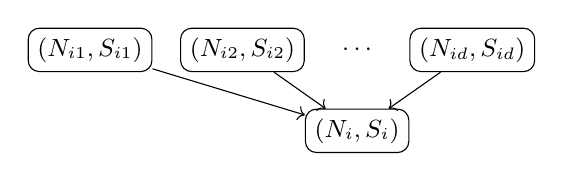
\begin{tikzpicture}[node distance=0.35cm,
                every node/.style={font=\small}]

                \node (s1) [draw, rounded corners] {$\left(N_{i1},S_{i1}\right)$};
                \node (s2) [draw, rounded corners, right=of s1] 
                    {$\left(N_{i2},S_{i2}\right)$};
                \node (dots) [right=of s2] {$\cdots$};
                \node (sd) [draw, rounded corners, right=of dots] 
                    {$\left(N_{id},S_{id}\right)$};

                \node (agg) [draw, rounded corners, below=0.55cm of dots]
                    {$\left(N_i,S_i\right)$};

                \draw[->] (s1) -- (agg);
                \draw[->] (s2) -- (agg);
                \draw[->] (sd) -- (agg);

            \end{tikzpicture}
            \end{center}

            \vspace{2mm} 

            \pause
            \alert{Shared secrets $S_i$ are independent}
            \pause

        \end{column}


        % ============================================================
        % RIGHT: Cascade derivation
        % ============================================================
        \begin{column}{0.48\textwidth}

            \begin{center}
                \textbf{Cascade Derivation} \color{LightHighlight}(in Sphinx)
            \end{center}

            \small
            \centering
            \vspace{2mm}

            % In Sphinx, \alert{cascade derivation} \vspace{2mm}\\
            $ s_1 \;\longrightarrow\; s_2 \;\longrightarrow\; \cdots \;\longrightarrow\; s_\ell $

            \vspace{1mm}

            \setlength{\fboxsep}{3mm}
            $$\color{LightHighlight}\boxed{\color{black} s_i = \textsf{Hash}\left(  r \: S_i \prod_{j=1}^{i-1} s_j  \right)}$$ %, \qquad i=1,\ldots,\ell $$

            \vspace{4mm}\pause

            Where $r$ is a nonce to rerandomize $\A{}$
            $$ \A{}' = r \: \A{} $$

            \vspace{2mm}
           
            \alert{ Fresh nonce $r$ \quad$\Rightarrow$\quad unlinkability}

        \end{column}

    \end{columns}

\end{frame}

\begin{frame}{Computation Time Across Protocol Stages}

    \vspace{7mm}
    \centering
    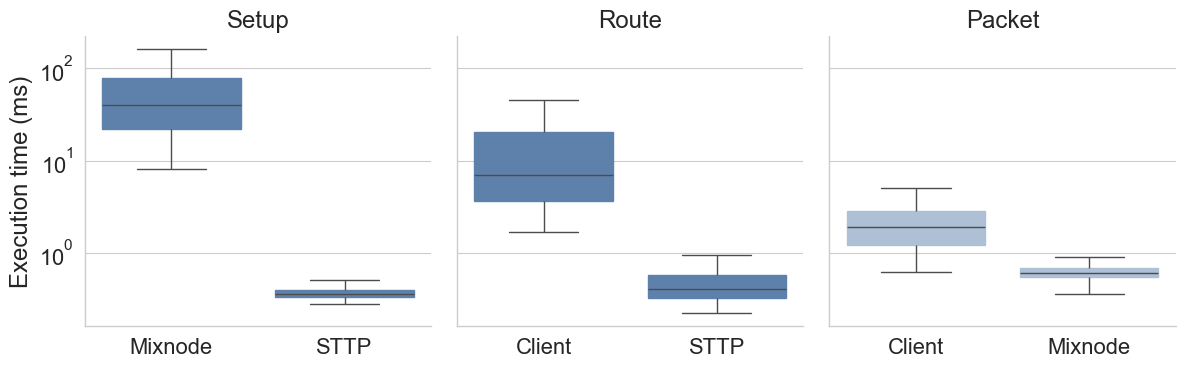
\includegraphics[width=\textwidth]{pictures/_boxplot.png}

    \vspace{8mm}

    \begin{center}
        \begin{tabular}{c@{\quad}c}
        \textbf{Overhead}
        &
        $\left\{
        \begin{minipage}{10cm}
            \begin{tabular}{cc}
                \textbf{Shamir secret sharing} & {\color{lightgray}(Mixnode Setup)} \\
                \textbf{Lagrange interpolation} & {\color{lightgray}(Client Aggregation)} \\ 
            \end{tabular}
        \end{minipage}
        \right.$
        \end{tabular}
    \end{center}
\end{frame}

\begin{frame}{Scalability with Respect to System Parameters}

    \vspace{3mm}
    \begin{columns}
        \begin{column}{0.5\textwidth}
            \centering
            \textbf{Route length}
            
            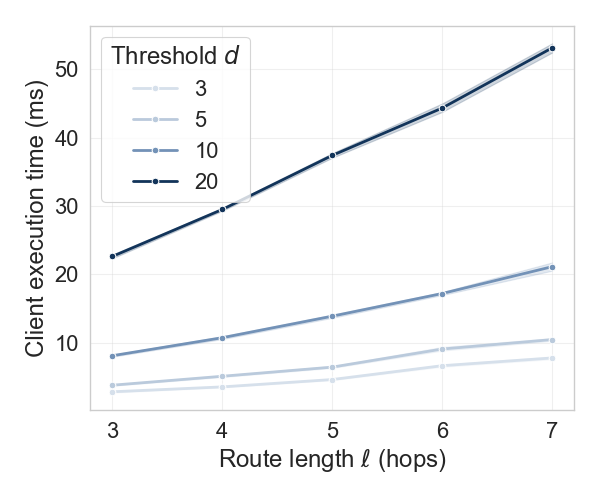
\includegraphics[width=\linewidth]{pictures/_path_length.png}
        \end{column}

        \begin{column}{0.5\textwidth}
            \centering
            \textbf{STTP threshold}
            
            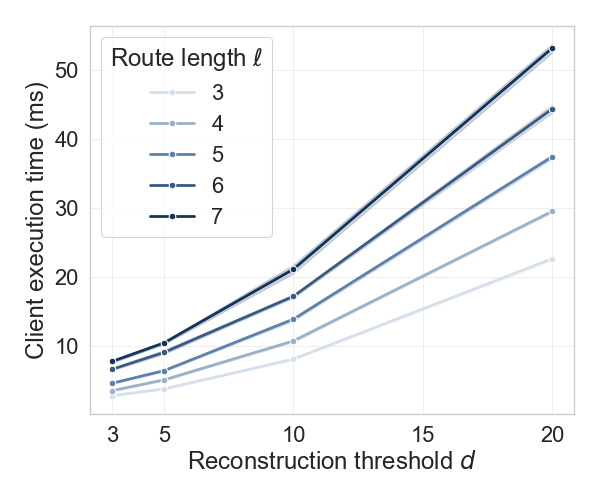
\includegraphics[width=\linewidth]{pictures/_threshold.png}
        \end{column}
    \end{columns}

    \vspace{5mm}

    \centering
    {\color{Highlight}Overhead remains moderate {\scriptsize\color{MidHighlight}(50 ms)} vs. end-to-end mixnet latency {\scriptsize\color{MidHighlight}(500-800 ms)}}
\end{frame}

\section{Conclusion}
\begin{frame}{Future Work}

\begin{itemize}
    \item[] \textbf{Alternative approaches}
    \hfill
    {\color{LightHighlight}ZK /VRF-based routing}

    \vspace{8mm}

    \item[] \textbf{Generalized route selection}
    \hfill
    {\color{LightHighlight}Cost-based routing}

    \vspace{8mm}

    \item[] \textbf{Broader applications}
    \hfill
    {\color{LightHighlight}Blockchain networks}
\end{itemize}

\end{frame}


\begin{frame}{Takeaway}

\begin{center}

\vspace{8mm}

\textbf{\Large Prevent route manipulation}\\[3mm]
{\color{LightHighlight}\large without compromising route privacy}

\vspace{12mm}

\begin{tabular}{c@{\hspace{8mm}}c@{\hspace{8mm}}c}
\textbf{Malicious client}
&
\multirow{2}{*}{$\longrightarrow$}
&
\textbf{Decentralized sampling}
\\
Route bias
&
&
Random route selection
\end{tabular}

\vspace{12mm}

\alert{Moderate overhead with preserved route confidentiality}

\end{center}

\end{frame}

\part{} % used to clean ToC later
\def\slidepart{0}
\begin{frame}[plain,noframenumbering,titlebackground]
    \maketitle
\end{frame}


%%% appendix
% \appendix

% \begin{frame}[plain, noframenumbering,nobackground]
% \begin{center}
% \LARGE Thank you for your attention.
% \vfill
% \LARGE Any Question?
% \end{center}
% \end{frame}

\end{document}


% My current works for my PhD are:

% 1) Decentralizing the route sampling procedure in mixnet to prevent malicious client from doing biased route based attacks to reduce anonymity of the system.
% 2) Extending and adapting the Sphinx packet format (used in mixnets) with Anonymous Destination-bound credential which allowed to verify at any mixnode that 
% the layered encrypted destination contained inside the packet is valid and authorized without leaking the source or final destination of the packet.
% This prevent abuse of the system to reach illegal / illicite web activities.

% As futur work, I would like to do one extra-work which would be focus en improving/enhancing those credentials.
% As for now, the credentials are only linked to a destination (and randomizable) but there is nothing to anonymously link it to a user, or prevent from "transferability" (i.e. copying and distributing the credential).
% Thus it makes to credential not yet interesting in practise (real-world scenario).
% Moreover, another problem in mixnet are unlimited client throughput. Imagine that a client can flood the system with lots of packets.
% Then he can DoS honest mixnodes, reduce the anonimity set of honest packets, and so on... 
% And in addition, it can make the first contribution less interesting (i.e. can ask random routes until having the route he wanted...).
% Therefore, to solve both the "non-transferability" and "flooding" problems, I would like to extend the credential with some kind of quota (i.e. rate-limiting, throughput regulation, maximal usages) without compromising privacy.



